\documentclass[11pt, oneside]{article}   	% use "amsart" instead of "article" for AMSLaTeX format
\usepackage[margin=1in]{geometry}                		% See geometry.pdf to learn the layout options. There are lots.
\geometry{letterpaper}                   		% ... or a4paper or a5paper or ... 
%\geometry{landscape}                		% Activate for rotated page geometry
%\usepackage[parfill]{parskip}    		% Activate to begin paragraphs with an empty line rather than an indent
\usepackage{graphicx}				% Use pdf, png, jpg, or eps§ with pdflatex; use eps in DVI mode
								% TeX will automatically convert eps --> pdf in pdflatex		
\usepackage{amssymb}
%usepackage{undertilde}
\usepackage[numbered,framed]{matlab-prettifier}

\usepackage[T1]{fontenc}
\usepackage{mathtools}  % loads »amsmath«
\usepackage{physics}
\usepackage{listings}


\setlength{\parskip}{0.5em}
\lstset{
	language=C,                % choose the language of the code
	numbers=left,                   % where to put the line-numbers
	stepnumber=1,                   % the step between two line-numbers.        
	numbersep=5pt,                  % how far the line-numbers are from the code
	backgroundcolor=\color{white},  % choose the background color. You must add \usepackage{color}
	showspaces=false,               % show spaces adding particular underscores
	showstringspaces=false,         % underline spaces within strings
	showtabs=false,                 % show tabs within strings adding particular underscores
	tabsize=2,                      % sets default tabsize to 2 spaces
	captionpos=b,                   % sets the caption-position to bottom
	breaklines=true,                % sets automatic line breaking
	breakatwhitespace=true,         % sets if automatic breaks should only happen at whitespace
	title=\lstname,                 % show the filename of files included with \lstinputlisting;
}


%SetFonts
\newcommand\Rey{\mbox{\textit{Re}}}

\title{\vspace{-6ex} Assignment 6- Hybrid MPI + MP + CUDA Programming \\ {CSCI 596: Scientific Computing \& Visualization}  \vspace{-2ex}}
\author{Anup V Kanale}
\date{\vspace{-2ex}\today}							% Activate to display a given date or no date

\begin{document}
\maketitle \vspace{-5ex}

The goal of this assignment is understand the basics of cuda through two examples-- for calculating the pair distribution function, and to calculate $\pi$.

\vspace{-2ex}
\section{Task I-- Pair-Distribution Computation with CUDA}
\vspace{-2ex}The pair distribution function (PDF) is the probability of finding any two atoms, which are a given distance $r$ apart, in a given volume. It is popularly used to measure the order, especially crystalline materials.

To compute the pdf, we fist calculate the histogram of atomic pair distances, i.e., calculate the distance between all pairs of atoms $i$ and $j$, say $r_{ij}$, put them in the appropriate `\textit{bins}' $\Delta r$ to generate a histogram. Note that the maximum distance between pairs under periodic boundary condition is the diagonal of half the simulation box. The algorithm is as follows: \\
\noindent \texttt{for all histogram bins i} \\
\indent	\texttt{nhist[i] = $0$}\\
\texttt{for all atomic pairs (i,j)} \\
\indent	\texttt{++nhist[$r_{ij}/r$]} \\
Once this histogram is obtained, the pdf may then be computed using the following formula:
	\begin{equation}
		g(r_k) = \frac{\text{nhist($k$)}}{2 \pi r_k^2 \Delta r \rho N}
	\end{equation}
where $r_k$ is the distance between two atoms, $\rho$ is the number density of atoms, $N$ is the total number of atoms. Notice that the obtaining the histogram involves computing distance between all pairs of atoms, which can get expensive with a large number of atoms. The parallel processing power of the GPUs was used to carry out these computations.

\begin{figure}[!htbp] \label{fig:pdf}
	\centering
	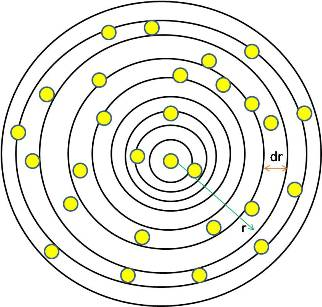
\includegraphics[scale=0.87]{pdf_pic.jpg}
	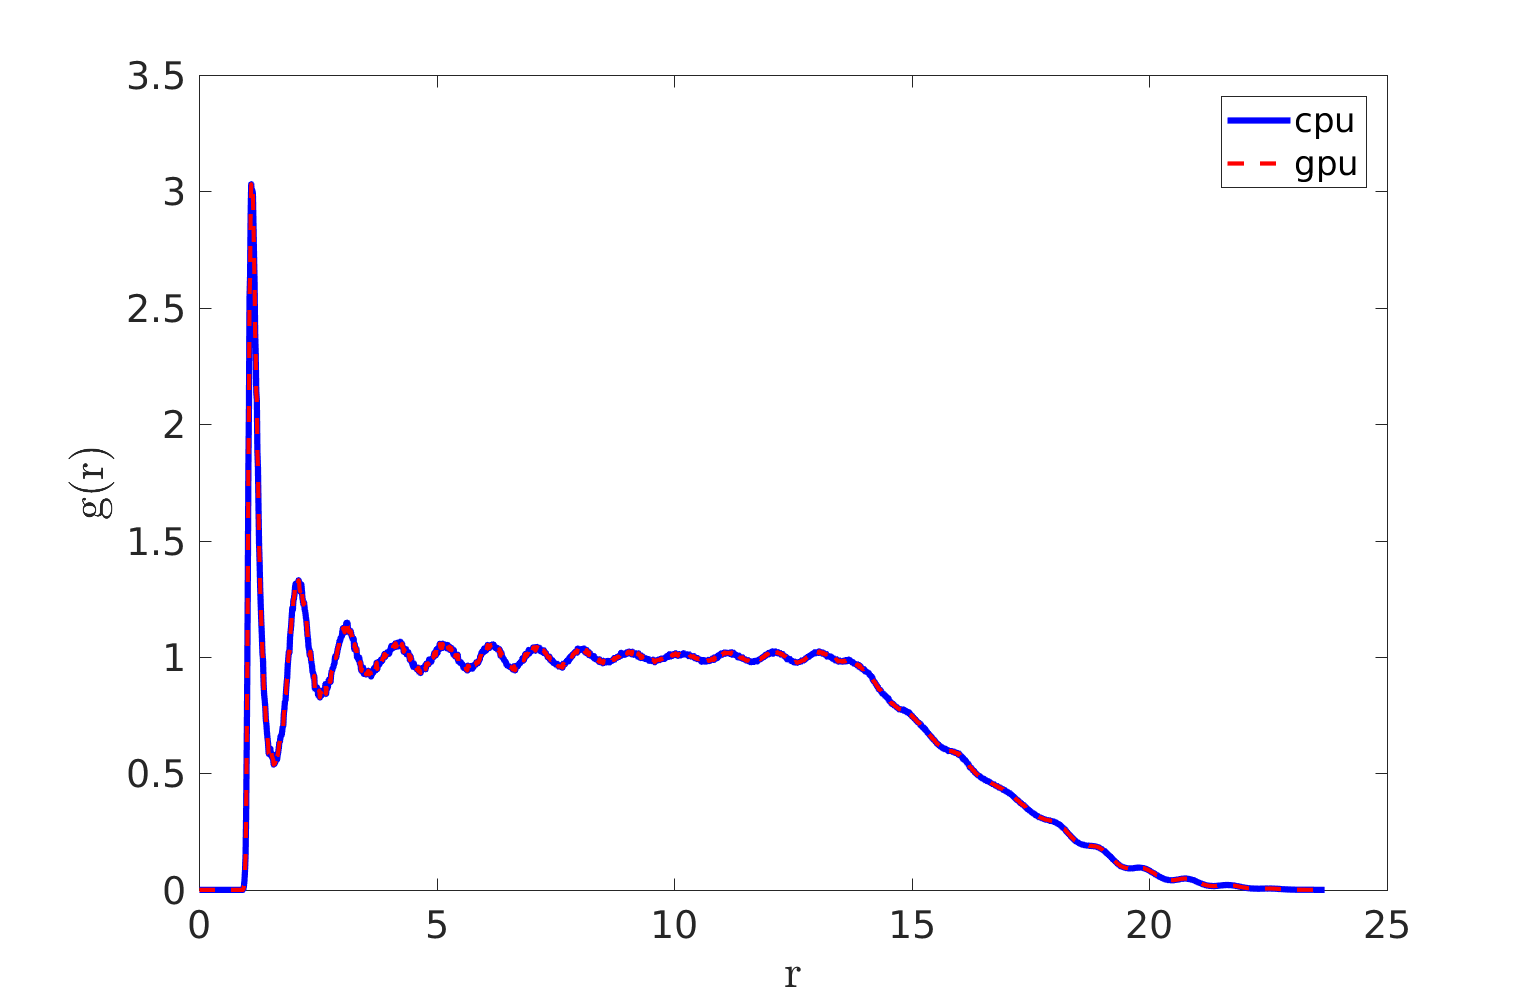
\includegraphics[scale=0.31]{pdf_cpuVsgpu.png}
	\caption{(a)Schematic for obtaining the histogram (b)PDF computation-- CPU vs GPU}
\end{figure}

The code is attached in Appendix A. The pair distribution function computed using both the CPU and the GPUs shown for comparison in Fig \ref{fig:pdf} (the trailing off after $r=14$ is explained in the notes.). The cpu implentation ran in 2.62 seconds whereas the gpu-parallel implementation ran in 0.28 seconds (almost 10 times faster!).



\vspace{-2ex}
\section{Task II-- Parallel Computation of $\pi$ using MPI+OMP+CUDA}
In this part, a triple-decker MPI+OpenMP+CUDA program was written to compute the value of $\pi$, by modifying the double-decker MPI+CUDA program provided in class, described in the lecture note on ``Hybrid MPI+OpenMP+CUDA Programming". The formula used is
	\begin{equation}
		\pi = \int_{0}^{1} \frac{4}{1+x^2} dx \approxeq \Delta \sum_{i=0}^{N-1} \frac{4}{1+x_i^2}
	\end{equation}

\begin{figure}[!htbp] \label{fig:piSchematic}
	\centering
	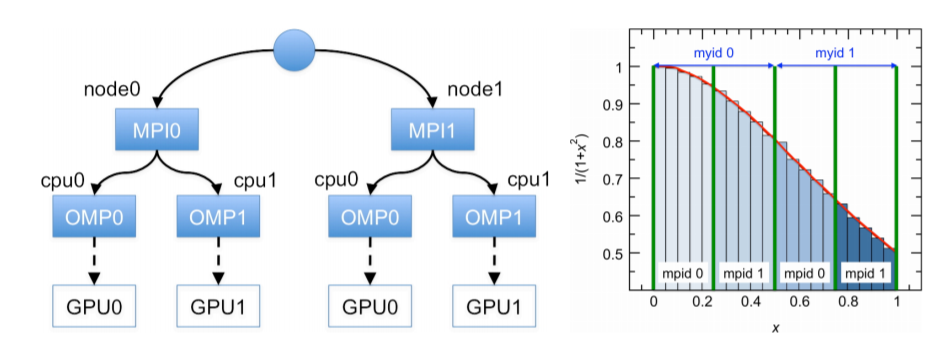
\includegraphics[scale=0.4]{piSchematic.png}
	\caption{Output of program for computation of $\pi$}
\end{figure}

This program runs on two CPU cores, and 2 GPU devices on each compute node. This is achieved by launching one MPI rank per node, where each rank spawns two OpenMP threads, and each thread uses a different GPU device. This is illustrated in Fig \ref{fig:piSchematic}. The above OpenMP multithreading introduces a race condition for variable pi. This can be circumvented by data privatization using \texttt{reduction(+:pi)}, which creates a \texttt{pi} variable for each thread. The `+:' means that the `addition reduction' is to be performed on this variable.

The program can be found in appendix B, and the output of the program is as shown below in Fig \ref{fig:pi}. \texttt{myid} refers to the process rank, \texttt{mpid} is the thread number within the processor, and \texttt{device used} refers to the gpu.
\begin{figure}[!htbp] \label{fig:pi}
	\centering
	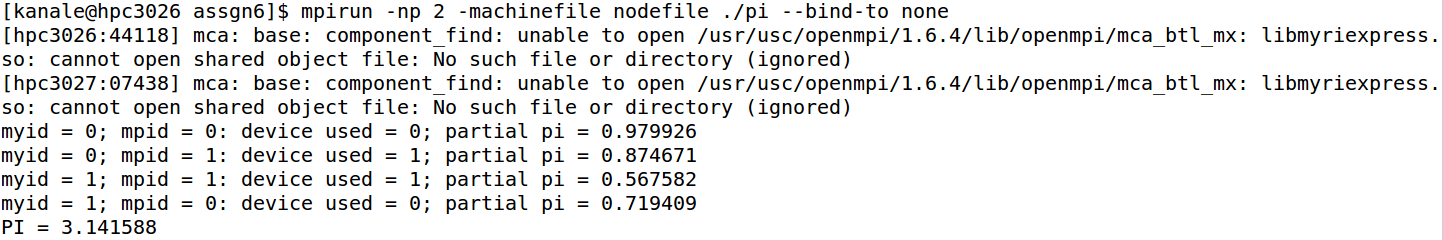
\includegraphics[scale=0.32]{piCalc.png}
	\caption{Output of program for computation of $\pi$}
\end{figure}

\textbf{Important points}\begin{enumerate}
 \item Finding compatible version of mpi, openMP and cuda is not trivial. And it varies from system to system.
 \item pay attention to how the sequential thread index is calculated across blocks.
\end{enumerate} 

\pagebreak
\appendix
\section{Appendix-- Calculating the PDF}
Note that there were no major changes in the \texttt{main()} function, so it is not shown.
\lstinputlisting{pdf1writeup.cu}

\section{Appendix-- Computation of $\pi$}
\lstinputlisting{piCudaMpiOmpwriteup.cu}

\end{document}